%%
%% FORMALIZATION
%%
\section{A Formal Notion of Transformation Networks}
\label{chap:correctness:formalization}

\mnote{Formalization of transformation networks and correctness}
We yet discussed a general notion of consistency and its preservation with a focus on a modular way of specifying it.
This notion was only specified in a rather informal way to first be able to discuss correctness notions and determine which notion is relevant for the considerations in this thesis.
In the following, we define a formal notion of consistency and its preservation, based on the informal explanation given before.
It extends the one we have presented in~\owncite{klare2020Vitruv-JSS}.
We also give a precise definition of notions for correctness between the artifacts of a modular specification.
Furthermore, we now focus on transformation-based approaches for preserving consistency, i.e., we consider specifications that transform changes within one or more models into changes in one or more other models, as a specialization of the general notion for consistency preservation that we have given before.

%Allgemeine Definition Transformationsnetzwerke:
%\begin{itemize}
    %\item Definition Transformation aus Relation und Wiederherstellungsroutinen; Routinen nehmen n Modelle und n Deltasequenzen (eine pro Modell) und liefern n Deltasequenzen zurück.
    %\item Im Allgemeinen könnte eine Transformation beliebige dieser Deltasequenzen modifizieren. Wir verlangen jedoch, dass eine Transformation nur Deltas anhängt, also die Sequenzen länger werden
    %\item Genauer beschränken wir auch, welche Sequenzen eine Transformation sehen und ändern darf, genau gesagt darf sie die Sequenzen von zwei Modellen sehen und eine davon verlängern.
    %\item Hier kommt bereits der Unterschied zu bisherigen Transformationen, denn die sehen nur Deltas an einem Modell und erzeugen Deltas an dem anderen. Das ist bei uns schon gänzlich anders. Bidirektionale Transformationen unterstützen das im Übrigen auch nicht, sondern sind nur Spezifikationen, aus denen sich Wiederherstellungsroutinen für beide Richtungen ableiten lassen (siehe Stevens 2010)
    %\item Relationen in erster Instanz auf Modellebene (also bzgl. ganzer Modelle, nicht einzelner Modellelemente) definieren
    %\item Direkt als multidirektionale Transformation definieren, also beliebig viele geändert Ein- und Ausgabemodelle (oder jeweils nur eins?)
    %\item Korrektheit einer Transformation (nach Stevens) definieren!
    %item Versuchen den Konkatenationsoperator zu definieren ohne dass er alle Metamodelle referenzieren muss (also Transformation wählt aus einer großen Eingabemenge relevanten Modelle aus, ändert relevante und dann fügt der Operator sie in die große Menge ein)
    %\item Definition Transformationsnetzwerk als Tupel aus Metamodellen, Transformationen und einer Ausführungsfunktion. 
    %\item Die Ausführungsfunktion führt für eine gegebene Änderung eine Auswahl der Transformationen nacheinander aus.
    %\item Korrektheit eines Netzwerkes definieren: Die Ausführungsfunktion erzeugt eine Transformationssequenz, die angewendet auf eine Änderung für alle Änderungen ein korrektes Ergebnisse produziert, d.h. die Modelle sind konsistent bzgl. allen Konsistenzrelationen.
%\end{itemize}


\subsection{Modular Consistency Specification}

\mnote{Extensional specifications are relations}
As already discussed informally before, an extensional specification of consistency enumerates all tuples of models that are considered consistent to each other, i.e., it specifies a relation between the models.

\begin{definition}[\ModelLevelConsistencyRelation]
    \label{def:modellevelconsistencyrelation}
    Given a tuple of metamodels $\metamodeltuple{M} = \tupled{\metamodelsequence{M}{n}}$, a \emph{\modellevelconsistencyrelation} $\consistencyrelation{CR}{}$ is a relation for instances of the metamodels $\consistencyrelation{CR}{} \subseteq \metamodeltupleinstanceset{M} = \metamodelinstanceset{M}{1} \times \dots \times \metamodelinstanceset{M}{n}$.

    For a tuple of models $\modeltuple{m} = \tupled{\model{m}{1}, \dots, \model{m}{n}} \in \metamodeltupleinstanceset{M}$ we say that:
    \begin{align*}
        \modeltuple{m} \consistenttomath \consistencyrelation{CR}{} \equivalentperdefinition \modeltuple{m} \in \consistencyrelation{CR}{}
    \end{align*}
    Otherwise, we call $\modeltuple{m} \inconsistenttomath \consistencyrelation{CR}{}$.
\end{definition}

\mnote{Start with coarse-grained model-level relations}
Given a tuple of models, we consider it consistent if it is contained in the consistency relation.
This conforms to consistency definitions such as the one proposed by \textcite{stevens2010sosym} for bidirectional transformations.
We explicitly denote this kind of consistency relation as \emph{model-level}, because we will later need to refine the notion of consistency relations to the level of \metaclasses and need to distinguish between the two.

\mnote{Modular notions of consistency}
If a single relation describes consistency between all relevant models, consistency is directly defined by means of model tuples being contained in that relation. We call such a relation a \emph{monolithic relation}.
However, if we have a \emph{modular} notion of consistency, i.e., a relation that does only define consistency between some of the relevant models and the global notion of consistency is defined by a combination of several such relations, we need an explicit definition for that notion.
For the sake of simplicity, we focus on binary relations as a modular representation of consistency, but this definition could also be generalized to relations of arbitrary arity.

\begin{definition}[Model-Level Consistency] 
    \label{def:modellevelconsistency}
    Let $\metamodeltuple{M} =  \tupled{\metamodelsequence{M}{n}}$ be a tuple of metamodels and let $\consistencyrelation{CR}{i,j} \subseteq \metamodelinstanceset{M}{i} \times \metamodelinstanceset{M}{j}$ be a binary \modellevelconsistencyrelation for any two metamodels $\metamodel{M}{i}, \metamodel{M}{j} \in \metamodeltuple{M}$. %\setted{\metamodelsequence{M}{n}}$.
    For a given tuple of models $\modeltuple{m} = \tupled{\model{m}{1}, \dots, \model{m}{n}} \in \metamodeltupleinstanceset{M}{}% = \metamodelinstanceset{M}{1} \times \dots \times \metamodelinstanceset{M}{n}
    $, we say that $\modeltuple{m}$ is \emph{consistent to} $\consistencyrelation{CR}{i,j}$ if, and only if, the instances of $\metamodel{M}{i}$ and $\metamodel{M}{j}$ are in that relation:
    \begin{align*} 
        &
        \modeltuple{m} %= \tupled{\model{m}{1}, \dots, \model{m}{n}} 
        \consistenttomath \consistencyrelation{CR}{i,j} \equivalentperdefinition %\\
        %& \formulaskip
        \tupled{\model{m}{i},\model{m}{j}} \in \consistencyrelation{CR}{i,j}
        %\exists \model{m}{i} \in \metamodelinstanceset{M}{i}, \model{m}{j} \in \metamodelinstanceset{M}{j} : \model{m}{i} \in \modelset{m} \land \model{m}{j} \in \modelset{m} \land \tupled{\model{m}{i}, \model{m}{j}} \in \consistencyrelation{CR}{}
    \end{align*}
    For a set of binary \modellevelconsistencyrelations $\consistencyrelationset{CR}$ for metamodels $\metamodeltuple{M}$, we say that a tuple of models $\modeltuple{m} \in \metamodeltupleinstanceset{M}{}$ is \emph{consistent to} $\consistencyrelationset{CR}$ if, and only if, it is consistent to each consistency relation in that set:
    \begin{align*} 
        &
        \modeltuple{m} \consistenttomath \consistencyrelationset{CR} \equivalentperdefinition %\\
        %& \formulaskip
        \forall \consistencyrelation{CR}{} \in \consistencyrelationset{CR} : \modeltuple{m} \consistenttomath \consistencyrelationset{CR}
    \end{align*}
\end{definition}

\mnote{Examplary binary relations}
The definition states that given a set of \modellevelconsistencyrelations the models must be consistent to all of these relations to consider them consistent to the set.
Consider, for example, the relations $\consistencyrelation{CR}{1} = \setted{\tupled{\model{m}{1}, \model{m}{2}}}$, $\consistencyrelation{CR}{2} = \setted{\tupled{\model{m}{2},\model{m}{3}}}$ and $\consistencyrelation{CR}{3} = \setted{\tupled{\model{m}{1}, \model{m}{3}}}$ with $\model{m}{i} \in \metamodelinstanceset{M}{i}$ for metamodels $\metamodel{M}{i}$. Then the model tuple $\tupled{\model{m}{1}, \model{m}{2}, \model{m}{3}}$ is consistent to these relations, because it is consistent to each of the binary relations.
These consistency relations are equivalent to a monolithic relation $\consistencyrelation{CR}{} = \setted{\tupled{\model{m}{1}, \model{m}{2}, \model{m}{3}}}$, because a model tuple $\modeltuple{m}$ is consistent to $\consistencyrelation{CR}{}$ exactly when it is consistent to $\setted{\consistencyrelation{CR}{1}, \consistencyrelation{CR}{2}, \consistencyrelation{CR}{3}}$.

\mnote{Relation uniqueness assumption}
For reasons of simplicity, we assume that there is only one consistency relation between each pair of metamodels.
This also includes that there are no two consistency relations $\consistencyrelation{CR}{i,j}$ and $\consistencyrelation{CR}{j,i}$ for metamodels $\metamodel{M}{i}$ and $\metamodel{M}{j}$, which means that the relations do not have a directionality.
This assumption is without loss of generality, because two relations between the same metamodels are, independent from their direction, equivalent to only considering their intersection, i.e., only the model pairs that are considered consistent by both relations.
%\todo{wlog: no direction of relation}

% \subsection{Expressiveness of Modular Consistency Specifications}
% \label{chap:correctness:formalization:expressiveness}

\mnote{Expressiveness of modular specifications}
Although in the preceding exemplary case the binary relations are equivalent to a monolithic relation, such an equivalence is not always given. In general, two interesting insights come along with that definition of consistency based on modular relations. First, expressiveness of defining consistency modularly by a set of relations is not equivalent to defining one monolithic relation between all models. Second, a modular definition of consistency can easily contain contradictions, which may lead to an empty tuple of consistent models.

\begin{figure}
    \centering
    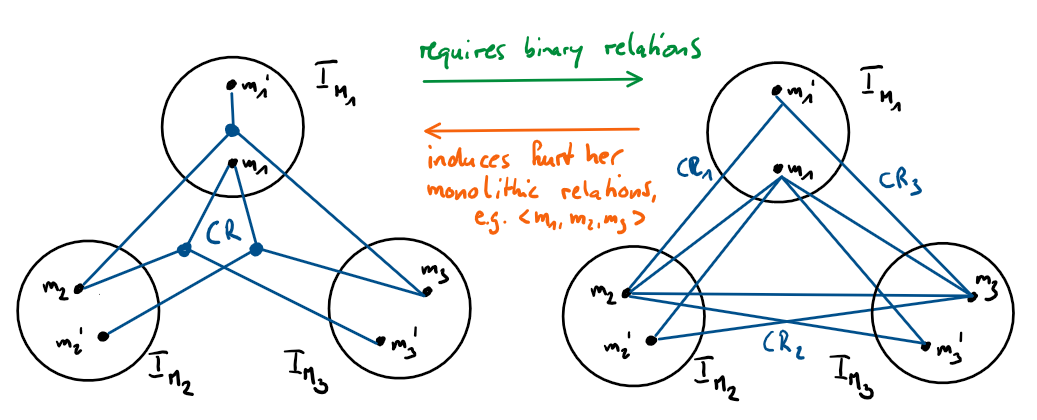
\includegraphics[width=\textwidth]{figures/correctness/notion/binary_definable.png}
    \caption[Monolithic consistency relation that cannot be modularized]{A monolithic consistency relation which cannot be expressed by binary relations.}
    \label{fig:correctness:binary_definable}
\end{figure}

\mnote{Binary relations reduce expressiveness}
It is easy to see that a combination of binary relations is not able to express the same consistency relations as one monolithic relation.
For example, the monolithic relation $\consistencyrelation{CR}{} = \setted{\tupled{\model{m}{1}, \model{m}{2}, \model{m}{3}'}, \tupled{\model{m}{1}, \model{m}{2}', \model{m}{3}}, \tupled{\model{m}{1}', \model{m}{2}, \model{m}{3}}}$ cannot be expressed by binary relations, as also depicted in \autoref{fig:correctness:binary_definable}.
The binary relations necessarily need to contain $\tupled{\model{m}{1}, \model{m}{2}}$ because $\tupled{\model{m}{1}, \model{m}{2}, \model{m}{3}'} \in \consistencyrelation{CR}{}$, $\tupled{\model{m}{1}, \model{m}{3}}$ because $\tupled{\model{m}{1}, \model{m}{2}', \model{m}{3}} \in \consistencyrelation{CR}{}$, and $\tupled{\model{m}{2}, \model{m}{3}}$ because $\tupled{\model{m}{1}', \model{m}{2}, \model{m}{3}} \in \consistencyrelation{CR}{}$. However, this would mean that $\tupled{\model{m}{1}, \model{m}{2}, \model{m}{3}}$ is considered consistent to the binary relations although it not consistent to the modular relation $\consistencyrelation{CR}{}$.
Thus, using sets of binary relations in contrast to a single monolithic relation reduces expressiveness.
\textcite{stevens2020BidirectionalTransformationLarge-SoSym} discusses the property of a multiary relation to be expressed by binary ones as \emph{binary-definable} in detail.
She proposes restrictions to binary relations that may be sufficient and still practical for expressing consistency, such as a notion of \emph{binary-implemented} relations.
However, we reasoned the assumption that relations need to be specified independently and thus modularly anyway, thus we have to accept that these restrictions in expressiveness exists.

\begin{figure}
    \centering
    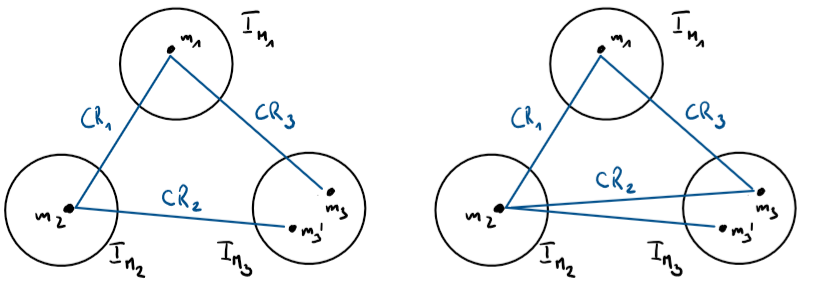
\includegraphics[width=\textwidth]{figures/correctness/notion/contradictions_example.png}
    \caption[Example for incompatible consistency relations]{Modular consistency relations, which together cannot be fulfilled (left) or which cannot be fulfilled for some of the consistent model pairs (right).}
    \label{fig:correctness:contradictions_example}
\end{figure}

\mnote{Contradictions of binary relations}
Additionally, it is easy to define multiple binary relations of which each can be fulfilled by certain models, but for which no tuple of models exists that is consistent to all of them. Consider the relations $\consistencyrelation{CR}{1} = \setted{\tupled{\model{m}{1}, \model{m}{2}}}$, $\consistencyrelation{CR}{2} = \setted{\tupled{\model{m}{2}, \model{m}{3}}'}$, $\consistencyrelation{CR}{3} = \setted{\tupled{\model{m}{1}, \model{m}{3}}}$, which are also depicted at the left of \autoref{fig:correctness:contradictions_example}.
Although for each of these relations a consistent tuple of models exists, which is exactly the one defined in each relation, no tuple of models exists that fulfills their combination.
This example already demonstrates the worst case, in which no consistent models exist for a set of relations.
In other cases, it may be possible that only for some models that are consistent according to one or some of the relations no model tuple exists that is consistent to all relations.
Consider the relations $\consistencyrelation{CR}{1} = \setted{\tupled{\model{m}{1}, \model{m}{2}}}$, $\consistencyrelation{CR}{2} = \setted{\tupled{\model{m}{2}, \model{m}{3}}, \tupled{\model{m}{2}, \model{m}{3}}'}$, $\consistencyrelation{CR}{3} = \setted{\model{m}{1}, \model{m}{3}}$, which are also depicted at the right of \autoref{fig:correctness:contradictions_example}.
In this case, the tuple $\tupled{\model{m}{1}, \model{m}{2}, \model{m}{3}}$ would be considered consistent to the relations, but although $\tupled{\model{m}{2}, \model{m}{3}'} \in \consistencyrelation{CR}{2}$ there exists no $\model{m^*}{1} \in \metamodelinstanceset{M}{1}$ so that $\tupled{\model{m^*}{1}, \model{m}{2}, \model{m}{3}'}$ is consistent to all these relations.

\mnote{Forbidden models through relations}
It is easy to see that one monolithic relation may be equally represented by an arbitrary number of sets of binary relations by simply adding model pairs to these binary relations that are never consistent to the other relations, like we have seen for the pair $\tupled{\model{m}{2}, \model{m}{3}}$ in the previous example.
This means that the combination of relations can lead to the situation that some models are actually forbidden (like $\model{m}{3}$ in the example before) due to the combination of consistency relations.
Whether such a situation is intended can eventually depend on the semantics of the actual models and relations, but we will discuss which situations may be unintended in general, independent from the scenario.
We already informally discussed this as a notion of \emph{compatibility}, for which we investigate in \autoref{chap:compatibility} how far this behavior is or should be expected.


\subsection{Incremental Consistency Preservation}
\label{chap:correctness:formalization:incremental_inductive}

\mnote{Preserving consistency}
While the previous discussion only considered when models are considered consistent, it is of especial interest to ensure that consistency of models is preserved.
We informally introduced such specifications as consistency preservation rules.
In the following, we will restrict us to \emph{incremental} and \emph{inductive} consistency preservation and give a precise definition for that.
This means that we make the following assumptions to the process.
\begin{properdescription}
    \item[Information Preservation (Incrementality):] After a change to one model, the others are not generated from scratch but updated according to the performed changes. This ensures that information that cannot be generated but was added by users to the other models is preserved.
    \item[Consistency Assumption (Induction):] We assume models to be consistent before a change is processed by consistency preservation rules. Otherwise, the preservation rules would need to be able to handle arbitrary states of the models and intentions of performed changes could not be incorporated to restore consistency.
\end{properdescription}
Incrementality is an essential requirement whenever consistency shall be preserved to avoid information loss. Otherwise, if for example Java code is always generated anew after changes to a \gls{UML} model instead of adapting it incrementally, all implementations of methods in Java get lost every time the \gls{UML} model is changed.
Inductivity, on the other hand, may not be necessary, as consistency preservation rules could also be defined to restore consistency from arbitrarily inconsistent states.
We, however, make this assumption to avoid requiring from the consistency preservation rules that they need to be able to process an inconsistent state without knowing which changes introduced it.
From a theoretical point of view, we could omit that requirement, but this would make the specification of consistency preservation rules impractically complicated, such that omitting that requirement is not practically relevant anyway.
%In consequence, an incremental and inductive \gls{consistency preservation rule} takes a consistent tuple of models and changes to them and returns a tuple of models that is consistent again.

%\todoLater{Do we need inductivity for synchronization? Otherwise we may remove it here and from following definitions?} % Yes, we do!
%\todo{Explicitly discuss incrementality here, although we actually do not need it. So leave it out? No, needed for synchronization definition. But make clear that this is a specialization and discuss generalization.}
%\todo{Make precise here that we have incremental consistency, thus last consistent state and delta to that is known. We did not assume that in the informal notion before.}

\mnote{Monolithic and modular consistency preservation}
Like we already discussed for consistency preservation rule in general, incremental preservation rules can be realized in an either monolithic or modular way.
A monolithic consistency preservation rules takes a tuple of models that is consistent to a consistency relation and a change to these models and returns another tuple of models that is consistent again.
In a modular specification of consistency preservation rules, a set of such rules is given which are able to preserve consistency of a subset of the given models according to modular consistency relations.
In our case, we consider such rules for two models, each of them restoring consistency according to a binary consistency relation.
%We will later discuss if and how an execution order of such consistency preservation rules can be determined.

\mnote{Drawbacks of existing consistency preservation approaches}
In the terminology for transformations, a consistency preservation rule that restores consistency of models according to a consistency relation in one direction is called \emph{directional transformation}~\cite{stevens2010sosym} or \emph{consistency restorer}~\cite{stevens2020BidirectionalTransformationLarge-SoSym}.
Definitions of that terminology do usually not consider changes but only states of models and simply define a consistency preservation rule $\consistencypreservationrule{}$ for metamodels $\metamodel{M}{1}$ and $\metamodel{M}{2}$ that modifies the instance of $\metamodel{M}{2}$ to restore consistency as:
\begin{align*}
    \consistencypreservationrule{}: \metamodelinstanceset{M}{1} \times \metamodelinstanceset{M}{2} \rightarrow \metamodelinstanceset{M}{2}
\end{align*}
This notion, however, has two properties that imply essential drawbacks:
\begin{properdescription}
    \item[State-based:] No information about the performed changes that led to the inconsistent state are given. This means that the specification is not aware of how the inconsistent state was reached.
    \item[Unidirectional:] The unidirectionality of the specification always requires to only update one model to restore consistency.
\end{properdescription}
State-based transformations always suffer from the problem that it is unknown which changes were made that led to an inconsistent state and reconstructing them from the difference between two states is only a heuristic approximation~\cite{diskin2011StateToDeltaSymmetric-MODELS}.
This, for example, includes that information about elements which were moved or renamed can potentially not be reconstructed, leading to elements that are deleted and created anew, losing all information that was potentially added to them.
Unidirectionality may be reasonable when assuming that only one of the models was modified. In that case it is sufficient to update the other model to restore consistency.
With a modular specification of consistency preservation, however, several consistency preservation rules modifying the same models may need to be executed.

\begin{figure}
    \centering
    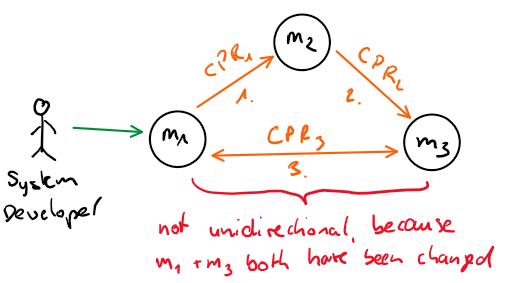
\includegraphics[width=0.7\textwidth]{figures/correctness/notion/not_unidirectional.png}
    \caption[Unidirectional consistency preservation in networks]{Consistency preservation rules of which at least one cannot be unidirectional because both models are modified by user or other consistency preservation rules.}
    \label{fig:correctness:unidirectionality_example}
\end{figure}

\mnote{Counterexample for unidirectionality}
\autoref{fig:correctness:unidirectionality_example} depicts an example why unidirectional consistency preservation rules cannot be applied of used in combination with others.
If the depicted consistency preservation rules $\consistencypreservationrule{1}$ and $\consistencypreservationrule{2}$ are executed first, $\consistencypreservationrule{3}$ cannot be unidirectional, as both involved models $\model{m}{1}$ and $\model{m}{3}$ have been modified either by the user or by another consistency preservation rule.
Thus, in general, it is not possible to only consider changes in one model and unidirectionally propagate them to the other model.
%\todo{add graphics and explanation for that; a simple example for a concurrent modification scenario (although maybe not induced by a network but several users) are that different classes are added to the UML and the Java model. Now it is necessary to react to changes in both models and to update both to reflect the classes added to the other. A single unidirectional transformation would result in reverting some changes, i.e., removing some classes that were added by the users}.
In consequence, the rules need to be able to deal with changes performed in both of the input models and, consequentially, need to update both models to reflect the changes in the other.

\mnote{Synchronizing consistency preservation rules}
To be able to combine several consistency preservation rules without the discussed drawbacks, we define a \emph{synchronizing} rather than a unidirectional notion of them.
Those rules are able to react to changes in both models and produce changes in both models again.
This is sometime also called the capability of handling \emph{concurrent} modifications (e.g. \cite{leblebici2014IncrementalTGGSurvey-GTVMT}).
To precisely define this behavior, we first introduce a notion of \emph{changes} and afterwards of \emph{consistency preservation rules}, which we also refer to as \emph{synchronizing} consistency preservation rules.

\mnote{Changes as functions}
As motivated before, we base our notion of consistency preservation on changes to explicitly express how a inconsistent state was derived from a previously consistent one.
We consider those changes to be functions that take a model and return a new one.
They are explicitly not defined for a specific model but for all instances of one metamodel.
This is reasonable, because a change is supposed to represent how specific elements are modified, such as adding, removing or modifying them.
Thus, they can be applied to any models containing these affected elements.
This is also how actual implementations, such as the in \gls{EMF} behave.
When the elements a change affects are missing a model, applying the change may fail.
This is why we consider the function describing a change to be partial.
We denote partiality by allowing the function to return $\bot$ to indicate inputs for which the function is undefined.
%\todo{Refine change notion to be partial, because not every change is necessarily applicable. Even if it could be, maybe it should not be.}
%\todo{Discuss that change (esp. partial notion) is reasonable because of practical realization: Changes in EMF define changes to elements. If that element is found in the model, it can be applied, if not, its behavior is undefined. This induces a function like we propose here, because a change can be applied to any instance of a metamodel, not only to one model.}
%\todo{Define how a change tuple can be applied to a tuple. Then update every complicated statement about applying a tuple to a tuple by a tuple notation with the short notation.}
\begin{definition}[Change]
    \label{def:change}
    Given a metamodel $\metamodel{M}{}$, a change $\change{\metamodel{M}{}}$ is a partial function that takes an instance of that metamodel and returns another one or $\bot$:
    \begin{align*}
        \change{\metamodel{M}{}}: \metamodelinstanceset{M}{} \rightarrow \metamodelinstanceset{M}{} \cup \setted{\bot}
    \end{align*}
    It encodes any kind of modification, which may be just an element addition, or removal, an attribute change and so on, or any composition of changes.
    We denote the identity change, i.e., the change that always returns the input model, as $\identitychange$:
    \begin{align*}
        \identitychange(x) \equalsperdefinition x
    \end{align*}
    We denote the universe of all changes in $\metamodel{M}{}$, i.e., all subsets of $\metamodelinstanceset{M}{} \times \metamodelinstanceset{M}{}$ that are functional, as:
    \begin{align*}
        \changeuniverse{\metamodel{M}{}} \equalsperdefinition \setted{\change{\metamodel{M}{}} \mid \change{\metamodel{M}{}} \subseteq \metamodelinstanceset{M}{} \times \metamodelinstanceset{M}{} \land
        (\tupled{\model{m}{1}, \model{m}{2}}, \tupled{\model{m}{1}, \model{m}{3}} \in \change{\metamodel{M}{}} \Rightarrow \model{m}{2} = \model{m}{3})}
    \end{align*}
    For a given metamodel tuple $\metamodeltuple{M} = \tupled{\metamodelsequence{M}{n}}$, we denote a tuple of changes to an instance of each metamodel as:
    \begin{align*}
        \changetuple{\metamodeltuple{M}} = \tupled{\change{\metamodel{M}{1}}, \dots, \change{\metamodel{M}{n}}}, \change{\metamodel{M}{i}} \in \changeuniverse{\metamodel{M}{i}}
    \end{align*}
    Likewise, we define the set of all tuples of changes in the instance tuples of 
    $\metamodeltuple{M}$, i.e. in $\metamodeltupleinstanceset{M}$, as $\changeuniverse{\metamodeltuple{M}}$:
    \begin{align*}
        \changeuniverse{\metamodeltuple{M}} \equalsperdefinition \changeuniverse{\metamodel{M}{1}} \times \dots \times \changeuniverse{\metamodel{M}{n}} %\setted{ \changetuple{\metamodeltuple{M}} = \tupled{\change{\metamodel{M}{1}}, \dots, \change{\metamodel{M}{n}}} \mid \forall i \in \setted{1,\dots,n} : \change{\metamodel{M}{i}} \in \changeuniverse{\metamodel{M}{i}} } 
    \end{align*}
    We define the application of a change tuple $\changetuple{\metamodeltuple{M}} = \tupled{\change{\metamodel{M}{1}}, \dots, \change{\metamodel{M}{n}}}$ to a model tuple $\modeltuple{m} = \tupled{\modelsequence{m}{n}} \in \metamodeltupleinstanceset{M}$ as the element-wise application of the changes:
    \begin{align*}
        \changetuple{\metamodeltuple{M}}(\modeltuple{m}) = \tupled{\change{\metamodel{M}{1}}(\model{m}{1}), \dots, \change{\metamodel{M}{n}}(\model{m}{n})}
    \end{align*}
\end{definition}

\mnote{Unapplicable changes}
For us, it does not matter how the function describing a change behaves in cases, in which the encoded change cannot be applied, e.g., because the changed or removed element does not exist. The function may do nothing for those models, i.e., return the identical model, or even be undefined for those model, i.e., be partial and return $\bot$.

\mnote{Reasonable change behavior}
In fact, we do restrict the actual behavior of a change in any way.
It may return an empty model, independent from the input, or may perform arbitrary changes to different models, instead of affects only specific elements.
We omit such restrictions, because they are not necessary for us, although, in practice, they are usually given.
Thus, further restricting the formalism would not provide any benefits.
%\todoLater{Check whether this behavior is correct.}

% \begin{definition}[\ModelLevelConsistencyPreservationRule]
%     Let $\metamodel{M}{1}, \metamodel{M}{2}$ be two metamodels and $\consistencyrelation{CR}{} \subseteq \metamodelinstanceset{M}{1} \times \metamodelinstanceset{M}{2}$ a binary \modellevelconsistencyrelation between them.
%     A \emph{\modellevelconsistencypreservationrule} $\consistencypreservationrule{\consistencyrelation{CR}{}}$ for the relation $\consistencypreservationrule{\consistencyrelation{CR}{}}$ is a function:
%     \begin{align*}
%         \consistencypreservationrule{\consistencyrelation{CR}{}} : (\metamodelinstanceset{M}{1}, \metamodelinstanceset{M}{2}, \change{\metamodel{M}{1}}) \rightarrow \change{\metamodel{M}{2}}
%     \end{align*}
%     It takes two consistent models and a change in the first one and returns a change in the second one.
%     We call a \modellevelconsistencypreservationrule \emph{correct} w.r.t. $\consistencyrelation{CR}{}$ if the resulting models when applying the input and output change are consistent to $\consistencyrelation{CR}{}$ again:
%     \begin{align*}
%         &
%         \forall \model{m}{1} \in \metamodelinstanceset{M}{1}, \model{m}{2} \in \metamodelinstanceset{M}{2} :
%         \tupled{\model{m}{1}, \model{m}{2}} \in \consistencyrelation{CR}{} \Rightarrow\\
%         & \formulaskip
%         \forall \change{\metamodel{M}{1}} \in \changeuniverse{\metamodel{M}{1}} :
%         \exists \change{\metamodel{M}{2}} \in \changeuniverse{\metamodel{M}{2}} :\\
%         & \formulaskip
%         \consistencypreservationrule{\consistencyrelation{CR}{}}(\model{m}{1}, \model{m}{2}, \change{\metamodel{M}{1}}) = \change{\metamodel{M}{2}} 
%         \land \tupled{\change{\metamodel{M}{1}}(\model{m}{1}), \change{\metamodel{M}{2}}(\model{m}{2})} \in \consistencyrelation{CR}{}
%     \end{align*}
% \end{definition}

\mnote{Consistency preservation rules}
With that notion of changes, we can define consistency preservation rules as functions receiving two models and changes to each own them and returning new changes to both models.

%\todo{Maybe remove \enquote{model-level} if we do not need a fine-grained notion of preservation rules. Maybe better call it \enquote{synchronizing} to be able to distinguish it from non-synchronizing ones later. -- No, not synchornizing, because other notion is only relevant in synchronization chapter, nowhere else.}
\begin{definition}[Consistency Preservation Rule]
    \label{def:consistencypreservationrule}
    Let $\metamodel{M}{1}, \metamodel{M}{2}$ be two metamodels and $\consistencyrelation{CR}{} \subseteq \metamodelinstanceset{M}{1} \times \metamodelinstanceset{M}{2}$ a binary \modellevelconsistencyrelation between them.
    A \emph{consistency preservation rule} $\consistencypreservationrule{\consistencyrelation{CR}{}}$ for the relation $\consistencyrelation{CR}{}$ is a function:
    \begin{align*}
        \consistencypreservationrule{\consistencyrelation{CR}{}} : (\metamodelinstanceset{M}{1}, \metamodelinstanceset{M}{2}, \changeuniverse{\metamodel{M}{1}}, \changeuniverse{\metamodel{M}{2}}) \rightarrow (\changeuniverse{\metamodel{M}{1}}, \changeuniverse{\metamodel{M}{2}}) \cup \setted{\bot}
    \end{align*}
    %It takes two consistent models and a change in the first one and returns a change in the second one. 
\end{definition}

\mnote{Partial consistency preservation rules}
For reasons of practical applicability, the rules need to be partial as we may not want to require them to be able to process arbitrary models and changes.
Like for changes, we denote this partiality by allowing the function to return $\bot$.
First, this is because we do not require it to produce any changes when the input models were not consistent.
Second, even if the input models are consistent, it may not be possible to preserve consistency for the given changes.
For example, if conflicting changes in both changes are made, i.e., changes that require one of them to be reverted, it may be desired that the consistency preservation rule does not return an unexpected result but to indicate a failure by returning $\bot$.
Our formalism does not restrict such a behavior, in fact it does even allow to always return the same changes or to return changes that always deliver empty models.
Finally, it is up to the developer to define reasonable consistency preservation rules and to define in which cases the function does not return a result.

\mnote{Conformance to existing definitions}
This notion of synchronizing consistency preservation conforms to the definition of \emph{synchronizers} given by \textcite{xiong2013SynchronizingConcurrentUpdates-SoSym}, which also reflect the case that both models have been modified and can be updated by the consistency preservation rule.
They do, however, encode the changes in terms of new model states rather than explicit changes.

\mnote{Correctness notion}
To consider a consistency preservation rule \emph{correct}, it has to return changes that, when applied to the input models, result in models that are consistent according to the \modellevelconsistencyrelation for which the preservation rule is defined.
This conforms to the notion of correctness defined for bidirectional transformations~\cite{stevens2010sosym} and the notion of consistency given for synchronizers by \textcite{xiong2013SynchronizingConcurrentUpdates-SoSym}.

%\todo{Revise such that the rule must not necessarily return a result (and also the definition of a rule itself), as it may be undefined for some inputs. Discuss that this is only a "can" requirement, so it is always possible to define a left-total CPR, because it can return any pair of consistent models (in the worst case always the same pair or the empty sets). We will later see that with other definitions this is a "must" requirement, but here we could, theoretically also require the CPR to always return a result. Nevertheless, practically we may want to support the case that the CPR cannot properly restore consistency for some inputs, e.g., because some of the input changes need to be reverted, which may not be wanted.
%Discuss that we do not define for which inputs the function may be undefined. It is up to the developer to reasonably use the ability to specify the function partially. In the extreme case, the function could be undefined for all inputs, which does not make sense, but thats up to the developer.}
\begin{definition}[Consistency Preservation Rule Correctness]
    \label{def:consistencypreservationrulecorrectness}
    Let $\consistencypreservationrule{\consistencyrelation{CR}{}}$ be a consistency preservation rule.
    We call $\consistencypreservationrule{\consistencyrelation{CR}{}}$ \emph{correct} if it either returns $\bot$ or changes that deliver models that are consistent to $\consistencyrelation{CR}{}$ if applied to the input models again:
    \begin{align*} &
        \consistencypreservationrule{\consistencyrelation{CR}{}} \correctmath \equivalentperdefinition %\\
        %& \formulaskip
        \forall 
        \model{m}{1} \in \metamodelinstanceset{M}{1}, 
        \model{m}{2} \in \metamodelinstanceset{M}{2},
        \change{\metamodel{M}{1}} \in \changeuniverse{\metamodel{M}{1}},
        \change{\metamodel{M}{2}} \in \changeuniverse{\metamodel{M}{2}} : \\
        & \formulaskip
        \bigl( \exists 
        \change{\metamodel{M}{1}}' \in \changeuniverse{\metamodel{M}{1}},
        \change{\metamodel{M}{2}}' \in \changeuniverse{\metamodel{M}{2}} :
        \consistencypreservationrule{\consistencyrelation{CR}{}}(\model{m}{1}, \model{m}{2}, \change{\metamodel{M}{1}}, \change{\metamodel{M}{2}}) = (\change{\metamodel{M}{1}}', \change{\metamodel{M}{2}}') \\
        & \formulaskip\formulaskip
        \Rightarrow
        \tupled{\change{\metamodel{M}{1}}'(\model{m}{1}), \change{\metamodel{M}{2}}'(\model{m}{2})} \consistenttomath \consistencyrelation{CR}{} \bigr)
        % &
        % \forall 
        % \model{m}{1} \in \metamodelinstanceset{M}{1}, 
        % \model{m}{2} \in \metamodelinstanceset{M}{2},
        % \change{\metamodel{M}{1}} \in \changeuniverse{\metamodel{M}{1}},
        % \change{\metamodel{M}{2}} \in \changeuniverse{\metamodel{M}{2}} :
        % \tupled{\model{m}{1}, \model{m}{2}} \consistenttomath \consistencyrelation{CR}{} \Rightarrow\\
        % & \formulaskip
        % \exists 
        % \change{\metamodel{M}{1}}' \in \changeuniverse{\metamodel{M}{1}},
        % \change{\metamodel{M}{2}}' \in \changeuniverse{\metamodel{M}{2}} :
        % \consistencypreservationrule{\consistencyrelation{CR}{}}(\model{m}{1}, \model{m}{2}, \change{\metamodel{M}{1}}, \change{\metamodel{M}{2}}) = (\change{\metamodel{M}{1}}', \change{\metamodel{M}{2}}') \\
        % & \formulaskip
        % \land \tupled{\change{\metamodel{M}{1}}'(\model{m}{1}), \change{\metamodel{M}{2}}'(\model{m}{2})} \consistenttomath \consistencyrelation{CR}{}
    \end{align*}
\end{definition}

\mnote{Reasonable consistency preservation rules}
This definition does not make any restrictions on how the input and output changes are related.
In fact, a valid (and especially correct) consistency preservation rule could always return empty changes.
In consequence, the rule would simply revert all input changes to achieve a consistent state again.
Although this may not be the expected behavior, there is no reason to restrict this behavior in the definition.
Actually, the developer of the preservation rule should specify in a \emph{reasonable} way, such that is provides any expected behavior.

%A \modellevelconsistencypreservationrule is defined to restore consistency after a modification in a left model of the underlying \modellevelconsistencyrelation by creating a change for the right model. To consider consistency preservation rules that preserve consistency in the other direction, we regard the inverse of the consistency relation as well, denoted as $\inverseconsistencyrelation{CR}{} = \setted{\tupled{\model{m}{1}, \model{m}{2}} \mid \tupled{\model{m}{2}, \model{m}{1}} \in \consistencyrelation{CR}{}}$.

\mnote{Transformations}
We already discussed that it is possible to define consistency relations and derive consistency preservation rules from them or to only define the consistency preservation rules, which then imply the consistency relations by their image, i.e., the set of all models that can be derived from applying the consistency preservation rule to any models and changes for which it is defined.
Anyway, in practice there will only be one of these specifications and the other is implied or derived.
We thus define a \emph{synchronizing transformation}, in extension to \emph{bidirectional transformations}~\cite{stevens2010sosym}, as an artifact that encapsulates a \modellevelconsistencyrelation together with a consistency preservation rule, no matter which of them is defined and which is derived or implied.

\begin{definition}[Synchronizing Transformation]
    \label{def:synchronizingtransformation}
    Let $\consistencyrelation{CR}{}$ be a \modellevelconsistencyrelation and $\consistencypreservationrule{\consistencyrelation{CR}{}}$ a consistency preservation rule that restores consistency according to that relation.
    A \emph{synchronizing transformation} is a pair $\transformation{t} = \tupled{\consistencyrelation{CR}{}, \consistencypreservationrule{\consistencyrelation{CR}{}}}$.
\end{definition}

\mnote{Transformation correctness}
Correctness of a transformation is then given by correctness of its consistency preservation rule.

\begin{definition}[Synchronizing Transformation Correctness]
    \label{def:synchronizingtransformationcorrectness}
    Let $\transformation{t} = \tupled{\consistencyrelation{CR}{}, \consistencypreservationrule{\consistencyrelation{CR}{}}}$ be a synchronizing transformation.
    We say that $\transformation{t}$ is correct if, and only if, $\consistencypreservationrule{\consistencyrelation{CR}{}}$ is correct according to \autoref{def:consistencypreservationrulecorrectness}:
    \begin{align*}
        &
        \transformation{t} \correctmath \equivalentperdefinition \consistencypreservationrule{\consistencyrelation{CR}{}} \correctmath
    \end{align*}
\end{definition}

\mnote{Hippocraticness}
Transformations are usually expected to by \emph{hippocratic}~\cite{stevens2010sosym}.
This means that a transformation, or more precisely its consistency preservation rule, does not perform any changes if the input changes applied to the input models already yield consistent models.
The application of hippocraticness to synchronizing transformations can be defined as follows.
\begin{definition}[Hippocratic Synchronizing Transformation]
    \label{def:hippocratictransformation}
    Let $\transformation{t} = \tupled{\consistencyrelation{CR}{}, \consistencypreservationrule{\consistencyrelation{CR}{}}}$ be a transformation for metamodels $\metamodel{M}{1}$ and $\metamodel{M}{2}$.
    We say that $\transformation{t}$ is \emph{hippocratic} if, and only if, it returns the input changes if their application to the input models yields consistent models:
    \begin{align*}
        &
        \transformation{t} \mathtextspacearound{hippocractic} \equivalentperdefinition
        \forall
        \model{m}{1} \in \metamodelinstanceset{M}{1}, \model{m}{2} \in \metamodelinstanceset{M}{2}, 
        \change{\metamodel{M}{1}} \in \changeuniverse{\metamodel{M}{2}}, \change{\metamodel{M}{2}} \in \changeuniverse{\metamodel{M}{2}} : \\
        &
        \tupled{\change{\metamodel{M}{1}}(\model{m}{1}), \change{\metamodel{M}{2}}(\model{m}{2})} \in \consistencyrelation{CR}{} \Rightarrow \consistencypreservationrule{\consistencyrelation{CR}{}}(\model{m}{1}, \model{m}{2}, \change{\metamodel{M}{1}}, \change{\metamodel{M}{2}}) = (\change{\metamodel{M}{1}}, \change{\metamodel{M}{2}})
    \end{align*}
\end{definition}

\mnote{Benefits of hippocraticness}
Although hippocraticness is not a necessary requirement for our considerations in most cases, it is usually a desired property in practice~\cite{stevens2010sosym}.
One benefit of hippocraticness with regards to transformations is given if a transformation is only defined by its consistency preservation rule and thus implies the underlying consistency relation as its fixed points, as discussed in \autoref{chap:correctness:notions_consistency:declarative_imperative}.
Actually, a consistency preservation rule according to our definition does not have fixed points, because the signatures of definition and value set of the function are different due to the models only occurring in the definition set.
Transferred to our definition, the consistency relation is implied by iteratively applying the function to each pair of models and changes with the changes delivered by the function until they are not modified by the function anymore.
In case that the transformation is correct and hippocratic, it does always deliver changes that yield consistent models already upon its first execution and does not modify them upon further applications, thus the consistency relation is implied by applying the function to each pair of models and changes only once.

\mnote{Generalization to transformations}
In the following, we will only refer to transformations rather than consistency relations and consistency preservation rules if the distinction is not necessary.
We will thus also say that models are consistent to a transformation, which is supposed to mean that they are consistent to the consistency relation encapsulated by that transformation.

\begin{definition}[Consistency to Transformation]
    \label{def:consistencytransformation}
    Let $\transformation{t} = \tupled{\consistencyrelation{CR}{}, \consistencypreservationrule{\consistencyrelation{CR}{}}}$ be a synchronizing transformation.
    We say that any tuple of models $\modeltuple{m}$ is \emph{consistent to} $\transformation{t}$ if, and only if, it is consistent to its consistency relation, i.e.
    \begin{align*}
        \modeltuple{m} \consistenttomath \transformation{t} \equivalentperdefinition \modeltuple{m} \consistenttomath \consistencyrelation{CR}{}.
    \end{align*}
    %
    For a set of transformations $\transformationset{T}$, we say that a model tuple $\modeltuple{m}$ is \emph{consistent to} $\transformationset{T}$ if, and only if, it consistent to all transformations in it, i.e.
    \begin{align*}
        \modeltuple{m} \consistenttomath \transformationset{T} \equivalentperdefinition \forall \transformation{t} \in \transformationset{T} : \modeltuple{m} \consistenttomath \transformation{t}.
    \end{align*}
\end{definition}

\mnote{Synchronization problem}
Although \autoref{def:synchronizingtransformationcorrectness} precisely defines when we consider a transformation to be correct, it is unclear how to define a transformation that fulfills such a correctness property.
In particular, most existing languages for specifying transformation are restricted to input changes to one model or at least to delivering changes to one model.
We will thus discuss how we can achieving a correct synchronizing transformation by means of such a restricted formalism.
This question was introduced as \autoref{rq:correctness:synchronization} and an approach for that constitutes our contribution \autoref{contrib:correctness:synchronization}, which we discuss in \autoref{chap:synchronization}.


\subsection{Transformation Orchestration}

\mnote{Multiple transformations need orchestration}
Having multiple transformations between several metamodels requires their orchestration, i.e., the decision which transformation have to be executed in which order, if consistency between instances of those metamodels shall be preserved after changes.
We discussed that transformations, or more precisely their consistency preservation rules, may be executed independently and thus concurrently, which requires their results to be unified, or to execute them consecutively.
We already identified the drawbacks of a concurrent execution approach, including the necessity to define unification operators and the missing guarantee to be consistent to any consistency relation after such a unification.
This is why we follow the approach of consecutively executing transformations.

\mnote{Orchestration function to determine execution order}
To consecutively execute transformations, an order of their execution has to be determined.
While in practice a dynamic algorithm will be used to determine that order, from a theoretical perspective that algorithm realizes a function that returns the order to execute the transformations in.
We call this an \emph{orchestration function} as it is responsible for orchestrating the execution of transformations.

%\todo{Prüfen, ob es valide ist, dass die Funktion nicht partiell ist. Man könnte bspw. sagen, die gibt im Fehlerfall einfach die leere Sequenz zurück. Dann müsste halt App prüfen, ob die Modelle schon konistent waren oder nicht.}
\begin{definition}[Transformation Orchestration Function] \label{def:orchestrationfunction}
    Let $\transformationset{T}$ be a set of transformations with consistency relations and according consistency preservation rules for metamodels $\metamodeltuple{M}$.
    A transformation orchestration function $\orcfunction{\transformationset{T}}$ for these transformations is a function that delivers a sequence of transformations for given models and changes:
    \begin{align*}
        &
        \orcfunction{\transformationset{T}} : (\metamodeltupleinstanceset{M}, \changeuniverse{\metamodeltuple{M}}) \rightarrow \transformationset{T}^{< \mathbb{N}}
    \end{align*}
    $\transformationset{T}^{< \mathbb{N}}$ denotes all finite sequences in $\transformationset{T}$, i.e., $\transformationset{T}^{< \mathbb{N}} \equalsperdefinition \emptyset \cup \transformationset{T}^1 \cup \transformationset{T}^2 \cup \dots$
\end{definition}

% \begin{definition}[Consistency Preservation Orchestration Function]
%     Let $\consistencypreservationruleset{}$ be a set of consistency preservation rules for a set of consistency relations $\consistencyrelationset{CR}$ on metamodels $\metamodeltuple{M} = \tupled{\metamodelsequence{M}{n}}$.
%     A consistency preservation orchestration function $\consistencyorcfunction{\consistencypreservationruleset{}}$ for these rules is a function:
%     \begin{align*}
%         &
%         \consistencyorcfunction{\consistencypreservationruleset{}} : (\metamodeltupleinstanceset{M}, \changeuniverse{\metamodeltuple{M}}) \rightarrow \consistencypreservationruleset{}^{< \mathbb{N}}
%     \end{align*}
%     $\consistencypreservationruleset{}^{< \mathbb{N}}$ denotes all finite sequences of consistency preservation rules in $\consistencypreservationruleset{}$, i.e., $\consistencypreservationruleset{}^{< \mathbb{N}} = \emptyset \cup \consistencypreservationruleset{}^1 \cup \consistencypreservationruleset{}^2 \cup \dots$.
% \end{definition}

\mnote{Repetitions in orchestration}
According to this definition, the orchestration functions returns a sequence of transformations and determines that their consistency preservation rules need to be executed in the given order. 
This especially includes that transformations may occur more than once in such a sequence.

\mnote{Existence of reasonable orchestrations}
It is obvious that without further restrictions to the transformations it is possible that, for given transformations, models and changes to them, an orchestration function cannot find an execution order that returns a consistent tuple of models after certain changes.
This can be because there is no such order, because the transformations make local decisions to restore consistency for two models that are in no case consistent with the other transformations.
Additionally, even if such an order exists, it may not be possible to find it.

% Consider the example in \autoref{fig:correctness:no_execution_order}. There exists no execution order for any input value that terminates. The transformations will always increase the value, although the defined relations could be fulfilled for the input value, but the transformations never find that solution.

% \begin{figure}
%     \centering
%     \includegraphics[width=\textwidth]{figures/correctness/notion/divergence_example.png}
%     \caption[Example for divergence]{Example for divergence}
%     \todo{Change caption}
%     \label{fig:correctness:no_execution_order}
% \end{figure}

\mnote{Decidability of existence of orchestration}
We will discuss these problems in detail in \autoref{chap:orchestration} and investigate whether we can find restrictions for the transformations that ensure that an orchestration that delivers a consistent result always exists.
We will also prove that without further restrictions the decision problem whether an orchestration exists that leads to a consistent result is undecidable.
Due to these degrees of freedom, the definition does not further restrict that an orchestration of transformations has to lead to a consistent result.

\mnote{Explicit function for transformation application}
An orchestration function does only determine an order of transformations.
Intuitively speaking, consistency for given models and changes to them can be preserved by requesting an orchestration from that function and executing the transformations in the given order.
We make this process explicit by defining an \emph{application function} that is able to perform consistency preservation based on given transformations, an orchestration function for them and the actual models and changes.

\mnote{Generalization function for transformation concatenation}
Before defining that application function, we first need to define an auxiliary function to concatenate transformations, more precisely their contained consistency preservation rules.
Consistency preservation rules according to \autoref{def:consistencypreservationrule} are restricted to the two metamodels they are defined for.
Additionally, they require initial models and changes as input, but only return changes.
For these two reasons, the functions describing the preservation rules cannot be easily concatenated.
This, however, is necessary to compose them to formally describe their consecutive execution.
We define a \emph{generalization function} for transformations, which generalizes them to arbitrary tuples of metamodels and a conforming signature for their input and output, which eases the description of their concatenation.

%\todo{Fix that transformation is a parameter and not index, rename function? We later have a generalization of consistency check}
%\todo{Correct that generalization function may return bot when the consistency preservation rule does. Update all usages of it appropriately}
%\todo{Update usages of generalization function to support the case when it return bot}
\begin{definition}[Transformation Generalization Function]
    \label{def:generalizationfunction}
    Let $\transformation{t} = \tupled{\consistencyrelation{CR}{}, \consistencypreservationrule{\consistencyrelation{CR}{}}}$ be a transformation for metamodels $\metamodel{M}{i}, \metamodel{M}{k}$.
    Let $\metamodeltuple{M} = \tupled{\metamodel{M}{1}, \dots, \metamodel{M}{i}, \dots, \metamodel{M}{k}, \dots, \metamodel{M}{n}}$ be a tuple of metamodels containing $\metamodel{M}{i}$ and $\metamodel{M}{k}$.
    A transformation generalization function $\generalizationfunction{\metamodeltuple{M},\transformation{t}}$ for metamodels $\metamodeltuple{M}$ and transformation $\transformation{t}$ is a partial function:
    \begin{align*}
        \generalizationfunction{\metamodeltuple{M},\transformation{t}} : (\metamodeltupleinstanceset{M}, \changeuniverse{\metamodeltuple{M}}) \rightarrow (\metamodeltupleinstanceset{M}, \changeuniverse{\metamodeltuple{M}}) \cup \setted{\bot}
    \end{align*}
    It generalizes the consistency preservation rule $\consistencypreservationrule{\consistencyrelation{CR}{}}$ of $\transformation{t}$ such that it can be applied to changes in $\metamodeltuple{M}$ instead of $\metamodel{M}{i}$ and $\metamodel{M}{k}$, i.e., it applies the changes delivered by $\consistencypreservationrule{\consistencyrelation{CR}{}}$ for the corresponding models to the given change tuple.
    Let $\modeltuple{m} \in \metamodeltupleinstanceset{M}$ be a model tuple and let $\changetuple{\metamodeltuple{M}} = \tupled{\change{\metamodel{M}{1}}, \dots, \change{\metamodel{M}{i}}, \dots, \change{\metamodel{M}{k}}, \dots, \change{\metamodel{M}{n}}}$ be a change tuple.
    We define $\tupled{\change{\metamodel{M}{i}}', \change{\metamodel{M}{k}}'} \equalsperdefinition \consistencypreservationrule{\consistencyrelation{CR}{}}(\model{m}{i}, \model{m}{k}, \change{\metamodel{M}{i}}, \change{\metamodel{M}{k}})$.
    Then the generalization function is defined as:
    \begin{align*}
        &
        \generalizationfunction{\metamodeltuple{M},\transformation{t}}(\modeltuple{m}, \changetuple{\metamodeltuple{M}}) \\
        &
        \formulaskip
        = 
        \begin{cases}
            \bot, & 
                \tupled{\change{\metamodel{M}{i}}', \change{\metamodel{M}{k}}'} = \bot \\
            (\modeltuple{m}, \tupled{\change{\metamodel{M}{1}}, \dots, \change{\metamodel{M}{i}}' %\concatfunction \change{\metamodel{M}{i}}
            , \dots, \change{\metamodel{M}{k}}'% \concatfunction \change{\metamodel{M}{k}}
            , \dots, \change{\metamodel{M}{n}}}), & 
                \otherwisemath
        \end{cases}
    \end{align*}
\end{definition}

% \begin{definition}[\ModelLevelConsistencyPreservationRule Generalization Function]
%     Let $\consistencypreservationrule{\consistencyrelation{CR}{}}$ be a \modellevelconsistencypreservationrule for metamodels $\metamodel{M}{i}, \metamodel{M}{k}$.
%     Let $\metamodeltuple{M} = \tupled{\metamodel{M}{1}, \dots, \metamodel{M}{i}, \dots, \metamodel{M}{k}, \dots, \metamodel{M}{n}}$ be a tuple of metamodels containing $\metamodel{M}{i}$ and $\metamodel{M}{k}$.
%     A \modellevelconsistencypreservationrule generalization function $\cprgeneralizationfunction{\consistencypreservationrule{\consistencyrelation{CR}{}}}$ is a function:
%     \begin{align*}
%         \cprgeneralizationfunction{\consistencypreservationrule{\consistencyrelation{CR}{}}} : (\metamodeltupleinstanceset{M}, \changeuniverse{\metamodeltuple{M}}) \rightarrow (\metamodeltupleinstanceset{M}, \changeuniverse{\metamodeltuple{M}})
%     \end{align*}
%     It generalizes $\consistencypreservationrule{\consistencyrelation{CR}{}}$ such that it can be applied to changes in $\metamodeltuple{M}$ instead of $\metamodel{M}{i}$ and $\metamodel{M}{k}$, i.e. it applies the changes delivered by $\consistencypreservationrule{\consistencyrelation{CR}{}}$ for the relevant models to the given change tuple.
%     Let $\modeltuple{m} \in \metamodeltupleinstanceset{M}$ be a model tuple and $\changetuple{\metamodeltuple{M}} = \tupled{\change{\metamodel{M}{1}}, \dots, \change{\metamodel{M}{i}}, \dots, \change{\metamodel{M}{k}}, \dots, \change{\metamodel{M}{n}}}$ a change tuple.
%     We define $\tupled{\change{m}{i}', \change{m}{k}'} \equalsperdefinition \consistencypreservationrule{\consistencyrelation{CR}{}}(\model{m}{i}, \model{m}{k}, \change{\metamodel{M}{i}}, \change{\metamodel{M}{k}})$.
%     Then the generalization function is defined as:
%     \begin{align*}
%         \cprgeneralizationfunction{\consistencypreservationrule{\consistencyrelation{CR}{}}}(\modeltuple{m}, \changetuple{\metamodeltuple{M}}) =
%         (\modeltuple{m}, \tupled{\change{\metamodel{M}{1}}, \dots, \change{\metamodel{M}{i}}' \concatfunction \change{\metamodel{M}{i}}, \dots, \change{\metamodel{M}{k}}' \concatfunction \change{\metamodel{M}{k}}, \dots, \change{\metamodel{M}{n}}})
%     \end{align*}
% \end{definition}

\mnote{Partial generalization function}
Like consistency preservation rules, a generalization function must also be partial, returning $\bot$ in cases it is undefined, to reflect cases in which it cannot return a result.
This is a direct consequence of consistency preservation rules being partial, thus a generalization function is defined to return $\bot$ in exactly those cases in which the consistency preservation rule is generalizes does so.

\mnote{Generalization function is universal}
The generalization function is a universally-defined auxiliary function that is only necessary to formalize the concepts.
It must neither be defined individually for a specific transformation, nor must it be explicitly specified by a developer of transformations at all.

\mnote{Dealing with unresolvable cases}
Finally, either the orchestration function or an application function must also be able to reflect the cases in which no execution order of transformation can be found that restores consistency.
In accordance to the terminology of \textcite{stevens2020BidirectionalTransformationLarge-SoSym}, we call those cases \emph{unresolvable}.
From a theoretical perspective, it does not make a difference whether the orchestration or the application function makes that decision. 
Finally, the orchestration function could also directly be encoded into the application function from a theoretical perspective.
However, from a practical perspective we may want to be able to find an execution order although there is no order that results in a consistent state, to be able to find out why it is not possible to restore consistency, thus, e.g., which transformation induces that problem.

\mnote{Application function}
We define a transformation application function that applies transformations to a given tuple of models and changes according to an order delivered by an orchestration function.
This function is partial to allow it to indicate that no result with consistent models could be found, e.g., because the input models were inconsistent or because a transformation within the orchestration delivered $\bot$.
We indicate those cases with the result $\bot$.

\begin{definition}[Transformation Application Function] \label{def:applicationfunction}
    Let $\transformationset{T}$ be a set of synchronizing transformations for consistency relations $\consistencyrelationset{CR}$ on metamodels $\metamodeltuple{M} = \tupled{\metamodelsequence{M}{n}}$ and $\orcfunction{\transformationset{T}}$ an orchestration function for them.
    A transformation application function $\appfunction{\orcfunction{\transformationset{T}}}$ for these rules is a partial function:
    \begin{align*}
        &
        \appfunction{\orcfunction{\transformationset{T}}} : (\metamodeltupleinstanceset{M}, \changeuniverse{\metamodeltuple{M}}) \rightarrow \metamodeltupleinstanceset{M} \cup \setted{\bot}
    \end{align*}
    The function takes a consistent tuple of models and a tuple of changes that was performed on them and returns a changed tuple of models by acquiring changes from the consistency preservation rules in $\consistencypreservationruleset{}$. %It is partial, because it is allowed to return $\bot$ especially for inconsistent input models but potentially also in other cases. 
    Thus, it has to fulfill the following condition:
    \begin{align*}
        &
        \forall \modeltuple{m} \in \setted{\modeltuple{m} \in  \metamodeltupleinstanceset{M} \mid \modeltuple{m} \consistenttomath \consistencyrelationset{CR}} : \forall \changetuple{\metamodeltuple{M}} \in \changeuniverse{\metamodeltuple{M}} : \\
        & \formulaskip
        \big( 
        %\appfunction{\orcfunction{\transformationset{T}}}(\modeltuple{m}, \changetuple{\metamodeltuple{M}}) = \bot \\
        %& \formulaskip 
        %\lor
            \exists \modeltuple{m'} \in \metamodeltupleinstanceset{M} : 
            \appfunction{\orcfunction{\transformationset{T}}}(\modeltuple{m}, \changetuple{\metamodeltuple{M}}) = \modeltuple{m'} \Rightarrow\\
            & \formulaskip \formulaskip
            \exists \transformation{t}_{1}, \dots, \transformation{t}_{m} \in \transformationset{T} :
            \exists \changetuple{\metamodeltuple{M}}' \in \changeuniverse{\metamodeltuple{M}} : %\\
            %& \formulaskip \formulaskip \formulaskip
            \orcfunction{\transformationset{T}}(\modeltuple{m}, \changetuple{\metamodeltuple{M}}) = \sequenced{\transformation{t}_{1}, \dots, \transformation{t}_{m}} \\
            & \formulaskip \formulaskip
            \land \generalizationfunction{\metamodeltuple{M},\transformation{t}_{1}} \concatfunction \dots \concatfunction \generalizationfunction{\metamodeltuple{M},\transformation{t}_{m}}(\modeltuple{m}, \changetuple{\metamodeltuple{M}}) = (\modeltuple{m}, \changetuple{\metamodeltuple{M}}') %\\
            %& \formulaskip \formulaskip \formulaskip
            \land \changetuple{\metamodeltuple{M}}'(\modeltuple{m}) = \modeltuple{m'}
        \big)
    \end{align*}
\end{definition}

\mnote{Weak notion of correctness}
While the previous definition does not restrict in which cases $\bot$ and in which an actual tuple of models is returned, we define when we consider an application function \emph{correct}.
Correctness can be defined in several ways.
For example, we might say that the function is correct if it returns a consistent tuple of models whenever there is an order of transformations that leads to those consistent models.
As we will see later, this is, however, generally impossible, because that decision problem is undecidable.
In consequence, the orchestration function and application function need to operate conservatively, i.e., return $\bot$ although there might be a sequence of transformations whose application leads to consistent models.
As an alternative, we might require the function to return consistent models whenever the orchestration function delivers a sequence of transformations whose application leads to a consistent tuple of models.
Since we have to deal with conservativeness anyway, this, however, does not provide any benefits.
In fact, the above discussed requirements encode a kind of \emph{optimality} for the functions, which we will specify more precisely in \autoref{chap:orchestration}.
For now, we stick to the simple notion of correctness that the application function does never return inconsistent models, i.e., if a tuple of models is returned, it must be consistent.

\begin{definition}[Transformation Application Function Correctness]
    \label{def:applicationfunctioncorrectness}
    Let $\appfunction{\orcfunction{\transformationset{T}}}$ be an application function for an orchestration function $\orcfunction{\transformationset{T}}$ for transformations $\transformationset{T}$.
    Let $\consistencyrelationset{CR}$ be the set of consistency relations for which the transformations in $\transformationset{T}$ are defined.
    We say that $\appfunction{\orcfunction{\transformationset{T}}}$ is \emph{correct} if, and only if, its result is either $\bot$ or consistent to $\consistencyrelationset{CR}{}$ for all inputs:
    \begin{align*}
        &
        \appfunction{\orcfunction{\transformationset{T}}} \correctmath \equivalentperdefinition %\\
        %& \formulaskip
        \forall \modeltuple{m} \in \metamodeltupleinstanceset{M} : \forall \changetuple{\metamodeltuple{M}} \in \changeuniverse{\metamodeltuple{M}} :
        \modeltuple{m} \consistenttomath \consistencyrelationset{CR} \\
        & \formulaskip
        \Rightarrow \appfunction{\orcfunction{\transformationset{T}}}(\modeltuple{m}, \changetuple{\metamodeltuple{M}}) = \bot \lor \appfunction{\orcfunction{\transformationset{T}}}(\modeltuple{m}, \changetuple{\metamodeltuple{M}}) \consistenttomath \consistencyrelationset{CR}
    \end{align*}
\end{definition}
% \begin{definition}[Consistency Preservation Application Function]
%     \todo{Define for transformations instead?}
%     Let $\consistencypreservationruleset{}$ be a set of consistency preservation rules for a set of consistency relations $\consistencyrelationset{CR}$ on metamodels $\metamodeltuple{M} = \tupled{\metamodelsequence{M}{n}}$ and $\consistencyorcfunction{\consistencypreservationruleset{}}$ an orchestration function for the consistency preservation rules.
%     A consistency preservation application function $\consistencyappfunction{\consistencypreservationruleset{}}$ for these rules is a partial function:
%     \begin{align*}
%         &
%         \consistencyappfunction{\consistencyorcfunction{\consistencypreservationruleset{}}} : (\metamodeltupleinstanceset{M}, \changeuniverse{\metamodeltuple{M}}) \rightarrow \metamodeltupleinstanceset{M} \cup \setted{\bot}
%     \end{align*}
%     The function takes a consistent tuple of models and a tuple of changes that was performed on them and returns a changed tuple of models by acquiring changes from the consistency preservation rules in $\consistencypreservationruleset{}$. It is partial, because it is allowed to return $\bot$ especially for inconsistent input models but potentially also in other cases. It has to fulfill the following conditions:
%     \begin{align*}
%         &
%         \forall \modeltuple{m} \in \metamodeltupleinstanceset{M} : \forall \changetuple{\metamodeltuple{M}} = \tupled{\change{\metamodel{M}{1}}, \dots, \change{\metamodel{M}{n}}} \in \changeuniverse{\metamodeltuple{M}} :
%         \modeltuple{m} \consistenttomath \consistencyrelationset{CR} \Rightarrow \\
%         & \formulaskip
%         \big( \consistencyappfunction{\consistencypreservationruleset{}}(\modeltuple{m}, \changetuple{\metamodeltuple{M}}) = \bot \\
%         & \formulaskip 
%         \lor
%             \exists \modeltuple{m'} \in \metamodeltupleinstanceset{M} : 
%             \consistencyappfunction{\consistencypreservationruleset{}}(\modeltuple{m}, \changetuple{\metamodeltuple{M}}) = \modeltuple{m'} \land\\
%             & \formulaskip \formulaskip
%             \exists \consistencypreservationrule{1}, \dots, \consistencypreservationrule{m} \in \consistencypreservationruleset{} : %\\
%             %& \formulaskip \formulaskip
%             \exists \changetuple{\metamodeltuple{M}}' = \tupled{\change{\metamodel{M}{1}}', \dots, \change{\metamodel{M}{n}}'} \in \changeuniverse{\metamodeltuple{M}} :\\
%             & \formulaskip \formulaskip
%             \consistencyorcfunction{\consistencypreservationruleset{}}(\modeltuple{m}, \changetuple{\metamodeltuple{M}}) = \tupled{\consistencypreservationrule{1}, \dots, \consistencypreservationrule{m}} \\
%             & \formulaskip \formulaskip
%             \land \cprgeneralizationfunction{\consistencypreservationrule{1}} \concatfunction \dots \concatfunction \cprgeneralizationfunction{\consistencypreservationrule{m}}(\modeltuple{m}, \changetuple{\metamodeltuple{M}}) = (\modeltuple{m}, \changetuple{\metamodeltuple{M}}')\\
%             & \formulaskip \formulaskip
%             \land \tupled{\change{\metamodel{M}{1}}'(\model{m}{1}), \dots, \change{\metamodel{M}{n}}'(\model{m}{n})} = \modeltuple{m'}
%         \big)
%     \end{align*}
%     We say that $\consistencyappfunction{\consistencyorcfunction{\consistencypreservationruleset{}}}$ is \emph{correct} if its result is either $\bot$ or consistent to $\consistencyrelation{CR}{}$:
%     \begin{align*}
%         &
%         \consistencyappfunction{\consistencypreservationruleset{}} \mathtext{is correct} \equivalentperdefinition \\
%         & \formulaskip
%         \forall \modeltuple{m} \in \metamodeltupleinstanceset{M} : \forall \changetuple{\metamodeltuple{M}} = \tupled{\change{\metamodel{M}{1}}, \dots, \change{\metamodel{M}{n}}} \in \changeuniverse{\metamodeltuple{M}} :
%         \modeltuple{m} \consistenttomath \consistencyrelationset{CR} \Rightarrow \\
%         & \formulaskip
%         \consistencyappfunction{\consistencypreservationruleset{}}(\modeltuple{m}, \changetuple{\metamodeltuple{M}}) = \bot \lor \consistencyappfunction{\consistencypreservationruleset{}}(\modeltuple{m}, \changetuple{\metamodeltuple{M}}) \consistenttomath \consistencyrelationset{CR}
%     \end{align*}
% \end{definition}

% The definition of the application function basically ensures that the function either returns $\bot$ or executes the \modellevelconsistencypreservationrules given by the orchestration function to retrieve a changes tuple of models.
% Actually, we want to have a notion of \emph{correctness}, because the function should not return a tuple of models that is not consistent.

% \begin{definition}[Correct Consistency Preservation Application Function]
%     Let $\consistencypreservationruleset{}$ be a set of consistency preservation rules for a set of consistency relations $\consistencyrelationset{CR}$ on metamodels $\metamodeltuple{M} = \tupled{\metamodelsequence{M}{n}}$ and $\consistencyorcfunction{\consistencypreservationruleset{}}$ an orchestration function for the consistency preservation rules.
%     We say that:
%     \begin{align*}
%         &
%         \consistencyappfunction{\consistencypreservationruleset{}} \mathtext{is correct} \equivalentperdefinition \\
%         & \formulaskip
%         \forall \modeltuple{m} \in \metamodeltupleinstanceset{M} : \forall \changetuple{\metamodeltuple{M}} = \tupled{\change{\metamodel{M}{1}}, \dots, \change{\metamodel{M}{n}}} \in \changeuniverse{\metamodeltuple{M}} :
%         \modeltuple{m} \consistenttomath \consistencyrelationset{CR} \Rightarrow \\
%         & \formulaskip
%         \consistencyappfunction{\consistencypreservationruleset{}}(\modeltuple{m}, \changetuple{\metamodeltuple{M}}) = \bot \lor \consistencyappfunction{\consistencypreservationruleset{}}(\modeltuple{m}, \changetuple{\metamodeltuple{M}}) \consistenttomath \consistencyrelationset{CR}
%     \end{align*}
% \end{definition}

\mnote{Conservativeness more relevant}
This, in fact, is a rather weak notion of correctness. 
Actually, an application function that always returns $\bot$ is correct according to that definition.
Due to the fact that the orchestration and application function have to operate conservatively, a binary correctness notion is not that relevant anyway.
Rather the degree of conservativeness, i.e., how often it returns no result although one exists, and how to improve it is of special interest.
The question how such an orchestration can or should look like was introduced as \autoref{rq:correctness:orchestration} and the degrees of freedom as well as a concrete approach will be presented as contribution \autoref{contrib:correctness:orchestration} in \autoref{chap:orchestration}.


\subsection{Transformation Networks}

\mnote{Transformation networks}
Based on the previous definitions of transformations, orchestration and application functions, we define what we consider a \emph{transformation network} and when we consider it \emph{correct}.
A transformation network is composed of transformations, an orchestration and an application function.
Although we define these artifacts specifically for one transformation network, i.e., an orchestration and application function according to their definitions is specific for one set of transformations, the goal will be to find an orchestration and application function that is independent from the actual transformations.

%\todo{Maybe also metamodels in transformation and networks?}
\begin{definition}[Transformation Network]
    \label{def:transformationnetwork}
    Let $\transformationset{T}$ be a set of transformations, $\orcfunction{\transformationset{T}}$ an orchestration function for these transformations and $\appfunction{\orcfunction{\transformationset{T}}}$ an application function.
    A transformation network $\transformationnetwork{N}$ is a triple:
    \begin{align*}
        \transformationnetwork{N} = \tupled{\transformationset{T}, \orcfunction{\transformationset{T}}, \appfunction{\orcfunction{\transformationset{T}}}}
    \end{align*}
\end{definition}

\mnote{Correctness of transformation networks}
Correctness of a transformation network is given by correctness of both the individual transformations as well as the application function, according to \autoref{def:synchronizingtransformationcorrectness} and \autoref{def:applicationfunctioncorrectness}.
We say that the transformations ensure \emph{local consistency}, because they are able to achieve consistency locally for two models, whereas the application function achieves \emph{global consistency} by applying the individual transformations in a ways such that all models are consistent according to all transformations afterwards.

\begin{definition}[Transformation Network Correctness]
    \label{def:transformationnetworkcorrectness}
    Let $\transformationnetwork{N} = \tupled{\transformationset{T}, \orcfunction{\transformationset{T}}, \appfunction{\orcfunction{\transformationset{T}}}}$ be a transformation network.
    We say that $\transformationnetwork{N}$ is \emph{correct} if, and only if, its transformations in $\transformationset{T}$ as well as the application function $\appfunction{\orcfunction{\transformationset{T}}}$ is correct:
    \begin{align*}
        & 
       \transformationnetwork{N} \correctmath \equivalentperdefinition %\\
        %& \formulaskip
        \forall \transformation{t} \in \transformationset{T} : \transformation{t} \correctmath \land \appfunction{\orcfunction{\transformationset{T}}} \correctmath
    \end{align*}
\end{definition}

\mnote{Conservativeness and compatibility}
We have already indicated that we will show that the application function has to operate conservatively, which is why correctness is an essential property, but not the most interesting one to achieve.
Additionally, we already suggested that the consistency relations of the transformations are considered correct by definition, as there is no other specification to which they have to be correct, but we will discuss a notion of \emph{compatibility} to reflect when those relations contain unintended contradictions.



%%% THIS VERSION MAKES ORCHESTRATION ON ITS OWN AND DEFINES THE REQUIREMENTS FOR THAT. IT MAY REQUIRE THE RESULT TO BE CONSISTENT OR NOT
% \begin{definition}[Consistency Preservation Application Function]
%     \todo{Define for transformations instead?}
%     Let $\consistencypreservationruleset{}$ be a set of consistency preservation rules for a set of consistency relations $\consistencyrelationset{CR}$ on metamodels $\metamodeltuple{M} = \tupled{\metamodelsequence{M}{n}}$.
%     A consistency preservation application function $\consistencyappfunction{\consistencypreservationruleset{}}$ for these rules is a partial function:
%     \begin{align*}
%         &
%         \consistencyappfunction{\consistencypreservationruleset{}} : (\metamodeltupleinstanceset{M}, \changeuniverse{\metamodeltuple{M}}) \rightarrow (\metamodeltupleinstanceset{M})
%     \end{align*}
%     The function takes a consistent tuple of models and a tuple of changes that was performed on them and returns a changed tuple of models by acquiring changes from the consistency preservation rules in $\consistencypreservationruleset{}$. It is partial, because it is only defined for consistent input model tuples and may not return a result for all possible changes to any model. It has to fulfill the following conditions:
%     \begin{align*}
%         &
%         \forall \modeltuple{m} \in \metamodeltupleinstanceset{M} : \forall \changetuple{\metamodeltuple{M}} = \tupled{\change{\metamodel{M}{1}}, \dots, \change{\metamodel{M}{n}}} \in \changeuniverse{\metamodeltuple{M}} :
%         \modeltuple{m} \consistenttomath \consistencyrelationset{CR} \Rightarrow \\
%         & \formulaskip
%         \exists \modeltuple{m'} \in \metamodeltupleinstanceset{M} :
%         \modeltuple{m'} = \consistencyappfunction{\consistencypreservationruleset{}}(\modeltuple{m}, \changetuple{\metamodeltuple{M}}) \\
%         %\land \modeltuple{m'} \consistenttomath \consistencyrelationset{CR} \\
%         & \formulaskip
%         \land \exists \consistencypreservationrule{1}, \dots, \consistencypreservationrule{m} \in \consistencypreservationruleset{} : 
%         \exists \changetuple{\metamodeltuple{M}}' = \tupled{\change{\metamodel{M}{1}}', \dots, \change{\metamodel{M}{n}}'} \in \changeuniverse{\metamodeltuple{M}} :\\
%         & \formulaskip \formulaskip 
%         \cprgeneralizationfunction{\consistencypreservationrule{1}} \concatfunction \dots \concatfunction \cprgeneralizationfunction{\consistencypreservationrule{m}}(\modeltuple{m}, \changetuple{\metamodeltuple{M}}) = (\modeltuple{m}, \changetuple{\metamodeltuple{M}}')\\
%         & \formulaskip \formulaskip
%         \land \tupled{\change{\metamodel{M}{1}}'(\model{m}{1}), \dots, \change{\metamodel{M}{n}}'(\model{m}{n})} = \modeltuple{m'}
%     \end{align*}
% \end{definition}


% It is obvious that we can define consistency preservation rules for which no execution order can be specified that returns a consistent tuple of models after certain changes. Consider the example in \autoref{fig:formal:noexecutionorder}. There exists no execution order for any input value that terminates. The transformations will always increase the value, although the defined relations could be fulfilled for the input value, but the transformations never find that solution.

% \begin{figure}
%     \centering
%     \includegraphics[width=\textwidth]{figures/correctness/formal/divergence_example.png}
%     \caption{Example for divergence}
%     \label{fig:formal:noexecutionorder}
% \end{figure}

% Although we will discuss restrictions to relations and transformations that reduce the chance that no solution can be found, it will not be possible to ensure that such a solution can always be found. This is due to the reason that transformations can perform arbitrary changes given the transformations Turing-completeness, which should not be restricted, because it is unclear which restrictions could be made without forbidding scenarios that should actually we supported. Thus, we assume that transformations are Turing complete.

% Finally, this makes it necessary that a function that applies \modellevelconsistencypreservationrules may not find an execution order that returns a consistent model, thus is should be able to also return $\bot$ as an indicator for that situation.

% We first give a basic definition for such a function without further specifying in which cases the function is expected to return a result other than $\bot$.

% \begin{definition}[Consistency Preservation Application Function]
%     \todo{Define for transformations instead?}
%     Let $\consistencypreservationruleset{}$ be a set of consistency preservation rules for a set of consistency relations $\consistencyrelationset{CR}$ on metamodels $\metamodeltuple{M} = \tupled{\metamodelsequence{M}{n}}$.
%     A consistency preservation application function $\consistencyappfunction{\consistencypreservationruleset{}}$ for these rules is function:
%     \begin{align*}
%         &
%         \consistencyappfunction{\consistencypreservationruleset{}} : (\metamodeltupleinstanceset{M}, \changeuniverse{\metamodeltuple{M}}) \rightarrow (\metamodeltupleinstanceset{M})
%     \end{align*}
%     The function takes a consistent tuple of models and a tuple of changes that was performed on them and returns a changed tuple of models by acquiring changes from the consistency preservation rules in $\consistencypreservationruleset{}$. Thus, it has to fulfill the following conditions:
%     {\setlength{\mathindent}{0em}
%     \begin{align*}
%         &
%         \consistencyappfunction{\consistencypreservationruleset{}}(\modeltuple{m}, \changetuple{\metamodeltuple{M}}) = 
%         \begin{cases}
%             \modeltuple{m'}, & \begin{array}{l@{}}
%                 \exists \changetuple{\metamodeltuple{M}}' = \tupled{\change{\metamodel{M}{1}}', \dots, \change{\metamodel{M}{n}}'} \in \changeuniverse{\metamodeltuple{M}} :\\
%                 \exists \consistencypreservationrule{1}, \dots, \consistencypreservationrule{m} \in \consistencypreservationruleset{} : \\
%                 \cprgeneralizationfunction{\consistencypreservationrule{1}} \concatfunction \dots \concatfunction \cprgeneralizationfunction{\consistencypreservationrule{m}}(\modeltuple{m}, \changetuple{\metamodeltuple{M}}) = (\modeltuple{m}, \changetuple{\metamodeltuple{M}}') \\
%                 \land \tupled{\change{\metamodel{M}{1}}'(\model{m}{1}), \dots, \change{\metamodel{M}{n}}'(\model{m}{n})} = \modeltuple{m'} 
%             \end{array} \\
%             \bot, & otherwise
%         \end{cases}
%     \end{align*}
%     }
% \end{definition}

% \begin{definition}[Consistency Preservation Application Function]
%     \todo{Define for transformations instead?}
%     Let $\consistencypreservationruleset{}$ be a set of consistency preservation rules for a set of consistency relations $\consistencyrelationset{CR}$ on metamodels $\metamodeltuple{M} = \tupled{\metamodelsequence{M}{n}}$.
%     A consistency preservation application function $\consistencyappfunction{\consistencypreservationruleset{}}$ for these rules is function:
%     \begin{align*}
%         &
%         \consistencyappfunction{\consistencypreservationruleset{}} : (\metamodeltupleinstanceset{M}, \changeuniverse{\metamodeltuple{M}}) \rightarrow (\metamodeltupleinstanceset{M})
%     \end{align*}
%     The function takes a consistent tuple of models and a tuple of changes that was performed on them and returns a changed tuple of models by acquiring changes from the consistency preservation rules in $\consistencypreservationruleset{}$. Thus, it has to fulfill the following conditions:
%     {\setlength{\mathindent}{1em}
%     \begin{align*}
%         &
%         \consistencyappfunction{\consistencypreservationruleset{}}(\modeltuple{m}, \changetuple{\metamodeltuple{M}}) = 
%         \begin{cases}
%             \modeltuple{m'}, & \begin{array}{l@{}}
%                 \exists \changetuple{\metamodeltuple{M}}' = \tupled{\change{\metamodel{M}{1}}', \dots, \change{\metamodel{M}{n}}'} \in \changeuniverse{\metamodeltuple{M}} :\\
%                 \exists \consistencypreservationrule{1}, \dots, \consistencypreservationrule{m} \in \consistencypreservationruleset{} : \\
%                 \cprgeneralizationfunction{\consistencypreservationrule{1}} \concatfunction \dots \concatfunction \cprgeneralizationfunction{\consistencypreservationrule{m}}(\modeltuple{m}, \changetuple{\metamodeltuple{M}}) = (\modeltuple{m}, \changetuple{\metamodeltuple{M}}') \\
%                 \land \tupled{\change{\metamodel{M}{1}}'(\model{m}{1}), \dots, \change{\metamodel{M}{n}}'(\model{m}{n})} = \modeltuple{m'} 
%             \end{array} \\
%             \bot, & otherwise
%         \end{cases}
%     \end{align*}
%     }
% \end{definition}



% \begin{definition}[Correct Consistency Preservation Application Function]
%     Let $\consistencyappfunction{\consistencypreservationruleset{}}$ be a consistency preservation application function for a set of \modellevelconsistencypreservationrules $\consistencypreservationruleset{}$ for a set of \modellevelconsistencyrelations $\consistencyrelationset{CR}$.
%     We say that:
%     \begin{align*}
%         &
%         \consistencyappfunction{\consistencypreservationruleset{}} \mathtext{is correct} \equivalentperdefinition \\
%         & \formulaskip
%         \forall \modeltuple{m} \in \metamodeltupleinstanceset{M} : \forall \changetuple{\metamodeltuple{M}} = \tupled{\change{\metamodel{M}{1}}, \dots, \change{\metamodel{M}{n}}} \in \changeuniverse{\metamodeltuple{M}} :
%         \modeltuple{m} \consistenttomath \consistencyrelationset{CR} \Rightarrow \\
%         & \formulaskip
%         \consistencyappfunction{\consistencypreservationruleset{}}(\modeltuple{m}, \changetuple{\metamodeltuple{M}}) \consistenttomath \consistencyrelationset{CR}
%     \end{align*}
% \end{definition}




%Now it is obvious that the consistency preservation rules can actually do anything to achieve consistency, including returning always the same set of models that is consistent, although that may not be expected. We will discuss later which reasonable assumptions can be made to the behavior to on the hand not restrict the possibilities of the transformation developer and on the other hand be able to ensure some properties of the transformations and their execution.


%Two levels of correctness:
%\begin{enumerate}
    %\item Local correctness: a consistency relation is correct to the global relation and the CPR is to the relation, i.e. given two models and changes in them, the transformation can produce a change that restores consistency regarding the global consistency relation of these two models (i.e. there are some other models with which these two models would be consistent regarding the global specification) --> a network is locally correct, if this property is fulfilled
    %\item Global correctness: the binary relations together are equal to the global one and the execution function is able to find consistency models after a change to initially consistent models --> network is globally correct, if this property is fulfilled
%\end{enumerate}
%Potentiell ist lokale Korrektheit (zumindest einer CPR zu ihrer CR per Konstruktion) herstellbar -- das war auch das Ergebnis bisheriger Studien --, eventuell auch von einer CR zu einer globalen CR, obwohl die ja eigentlich meist nicht existiert, daher nehmen wir das als gegeben an.
%Dann zeigen, dass die globale Beziehung der Relationen nicht äquivalent ist zu den einzelnen lokalen, daher kommt hier zusätzliche Komplexität rein (Kompatibilitätsbegriff).
%Final muss noch die Ausführungsfunktion korrekt sein, hier aber Problem der Turing-Vollständigkeit. 
%Daher Einschränkungen an Transformationen finden bzw. ingenieurmäßige Ausführungsreihenfolge festlegen, die möglichst oft richtige Lösungen findet und sonst konservativ mit einem Fehler terminiert.


% \textbf{On top of ordinary bx correctness:}
% \begin{itemize}
    %\item Transformations need to be synchronizing
    %\item Consistency relations need to fulfill a notion of correctness
    %\item Exkurs:
    % \begin{itemize}
    % %\item Is compatibility a subclass of correctness? Is every correct set of relations compatible as well?
    % \item Problematisch: unser Konsistenzbegriff für Relationen (feingranulare Relationen) schließt keine Modelle aus, der Konsistenzbegriff hier aber schon. Wie realisiere ich die feingranularen Relationen, die dafür sorgen, dass nur genau ein Tupel von Modellen konsistent ist?
    % \item Wir müssen bei der Ableitung unseres Kompatibilitätsbegriffes erklären, dass bei uns der vollständige Ausschluss bestimmter Modelle nicht Teil einer feingranularen Konsistenzrelation sein darf, sondern Teil einer weiteren Spezifikation, die angibt, welche Modelle überhaupt valide sind. Denn so ist es in Transformationssprachen tatsächlich auch.
    % \end{itemize}
    %\item Execution function needs to be defined, which potentially induces requirements to the transformations.
% \end{itemize}


% Voraussetzungen:
% \begin{itemize}
%     \item Relationen müssen korrekt sein, d.h. sie müssen bzgl. einer globalen (meist eher implizit bekannten) n-ären Relation zwischen allen Modellen identisch sein. Eine n-äre Relation lässt sich nicht immer zerlegen (siehe Stevens), aber wir nehmen das an.
%     \item Die einzelne Transformation muss bzgl. ihrer Relation korrekt sein, d.h. sie muss bei Änderungen in beiden Modellen ein zur Relation konsistentes Modell liefern.
% \end{itemize}

%Ebenen der Korrektheit:
%\begin{itemize}
    %\item Relationen müssen korrekt sein, d.h. gegeben eine Nutzeränderung muss es überhaupt möglich sein eine konsistente Menge an Modellen zu finden. Wenn Transformationen etwas beliebigen tun dürfen geht das immer. Wir nehmen an, dass eine Nutzeränderung nicht rückgängig gemacht werden soll (bzw. wenn sie rückgängig gemacht werden würde eigentlich die Änderung invalide war, d.h. keine Konsistenz im Netzwerk hergestellt werden kann). Daher sind Relationen nur korrekt, wenn für fixierte Elemente, die durch eine Nutzeränderung entstehen können, eine Modellmenge abgeleitet werden kann, die bzgl. der Relationen konsistent ist. D.h. gegeben einige Elemente muss es eine Modellmenge geben, die in allen Relationen liegt und die diese Elemente enthält (-> Kompatibilitätsbegriff). Wir betrachten in Kapitel ?, wie man Kompatibilität präzise definieren und feststellen/garantieren kann.\\
    %Resultat: Gegeben eine Änderung ist es möglich eine Transformation anzugeben, die aus der Änderung ein konsistentes Modell produziert.
    %\item Einzelne Transformationen müssen korrekt sein: Wir fordern Korrektheit der Transformation sowieso. Allerdings machen in einem Netzwerk verschiedene Transformationen Änderungen an allen Modellen, d.h. wir müssen nicht den "normalen" Transformationsfall unterstützen, dass Deltas in einem Modell ins andere übertragen werden, um Konsistenz herzustellen, sondern die Transformationen müssen \emph{synchronisierend} sein, also Deltas in beiden Modelle annehmen und dann Konsistenz herstellen. Wir definieren diese Synchronisationseigenschaft und betrachten in Kapitel ?, welcher zusätzlichen Anforderungen sich dadurch bzgl. EMOF-Modellen ergeben. Der Input sind Deltas in zwei Modellen, und einzelne Deltas sind potentiell als "authoritative" definiert, was bedeutet, dass die erzeugten/geänderten Elemente nicht noch einmal geändert/gelöscht werden dürfen. Das realisiert die Anforderung, dass Nutzeränderungen nicht rückgängig gemacht werden dürfen. \\
    %Resultat: Gegeben Änderungen in zwei Modellen (mit potentiell authoritativen Änderungen) gibt die Transformation ein konsistentes (bzgl. der Konsistenzrelation) Modellpaar zurück. 
    %\item Korrektheit der Anwendungsfunktion: Die Anwendungsfunktion muss die Transformationen in einer 
%\end{itemize}


% \todo{Überlegen, wo hier die Definition von (undirektionalen Relationen) rein muss.}
% Präzisere Eigenschaften:
% \begin{itemize} 
%     \item Synchronisationseigenschaft: Eine Transformation kann mit Änderungen an mehreren Modellen umgehen, d.h. gegeben zwei konsistente Modelle + Änderungen an beiden resultiert in zwei Modellen, die konsistent bzgl. der Relation(en) zwischen den Metamodellen sind
%     \item 
% \end{itemize}  

% \begin{itemize}
%     \item Kompatibilität entsprechend Modularisierungsebene
%     \item Synchronisation auf Operationalisierungsebene: Abwägen, dass eine Transformation verschiedene Zustände sehen könnte, auf denen sie ausgeführt wird. Aber letztendlich muss sie damit klarkommen, dass zwei Modelle geändert wurden. 
% \end{itemize}

%TODO:
%\begin{itemize}
    %\item Authoritative Modelle (bzw. eher authoritative Regionen) diskutieren (Verweis Stevens)
%\end{itemize}



% \section{Local Correctness}

% Simple solution: we define a transformation which normatively implies a relation, thus it is correct by construction. From a theoretical perspective this is easy to reach, from a practical it is not.
% However, in contrast to our definition of synchronizing transformations, ordinary transformations are only able to process changes in one model and update the other accordingly. Together with the assumption that both models were consistent before does not fit with our scenario, because if one model is modified, the other may be modified as well by another transformation across another path, before a transformation is executed. Thus, both models may have been modified.
% We consider the following situation: Models A and B were consistent. Model A was changed an we have the changes at hand. Additionally, B was modified because there were other changes propagated through the network. 
% We distinguish all cases of modifications to B that may have violated a consistency relation between A and B (according to our fine-grained consistency notion) and consider what we have to do there (e.g. find-or-create-pattern).
% Put empirical analysis here.


% \section{Correct APP function}

% We make the following approach: Always assume there is a solution and start executing the transformation (for now in any order). Finally, the network has to terminate at a fixed point. We investigate, what the reasons may be that it does not try to avoid them.

% These reasons can lie in the relations:
% - relations cannot be completely unfulfillable, as the empty models are always consistent, thus there can always be CPRs that result in a consistent set of models
% - however, if relations contain pairs that can never be in any consistent model tuple they improve proneness to errors, because a CPR may return that pair, which will never fit to any result of any other transformation. Thus, this should not be allowed -> compatibility

% These reasons can also lie in the transformations:
% - Transformations can make choices and they make choices that are always incompatible to other (refer to example)

% Essentially there are two problems: alternation and divergence


% \subsection{Other thought}
% If each element occurs in each relation only once (so always 1:1 mappings) and if we have compatibility, then any transformation order would return exactly the one model tuple that fits.
% However: In that case we would have confluence, every information must directly be available in B from A without a transitive propagation over C. This is not what we want. So there must in general be more than one option a transformation is fine with that to reflect the information that another transformation may add or change.


%\todo{Hippocraticness is not necessary but needs to be discussed}

% Goal:
% - Find a solution in as much cases as possible, abort in the others (conservatively)
% - To do so: reduce cases in which there is no such function
% - To do so: ensure that relations are defined in a way such that they do not allow a locally correct set of CPRs that has no APP solution. If there is a pair of models (or elements of a fine-grained relation) in a relation, a CPR may return it. But if there is no consistent tuple of models containing these two, it does not make any sense to consider these elements (even worse, if we have monotony, adding these elements makes the network unsolvable). For that reason, we need compatibility.
